\documentclass{standalone}
\usepackage{hsbcommon}
%% Show/hide steps for standalone work — edit this line:
\makeatletter\AtBeginDocument{\@buildstepset{0,1,2,3,4}}\makeatother
\begin{document}
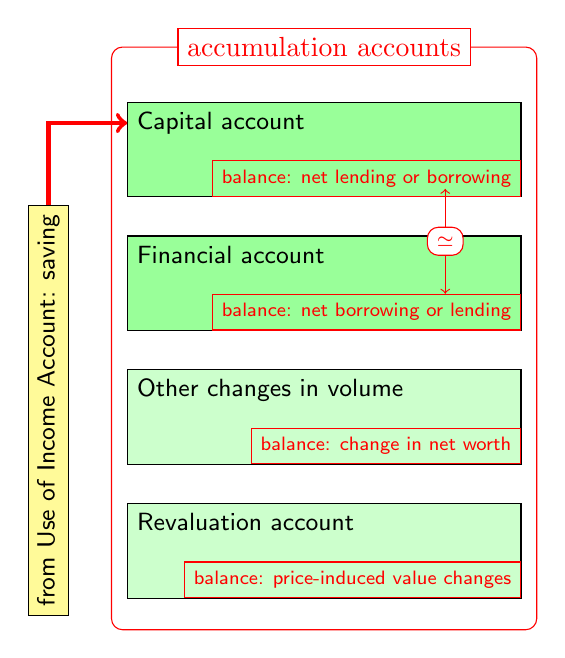
\begin{tikzpicture}
    \def\mystretch{1.7}
    \tikzset{
        myaccount/.style={
            draw,
            font=\small\sffamily
        } 
    }
    \foreach[count=\i] \myaccount/\mybalance/\mycolor in 
        {%
        Capital account/net lending or borrowing/green!40,
        Financial account/net borrowing or lending/green!40,
        Other changes in volume/change in net worth/green!20,
        Revaluation account/price-induced value changes/green!20%
        }
        {
            \ifstep{\i}{
                \draw[myaccount,fill=\mycolor] (0,-\mystretch*\i) 
                    node[below right] (A\i) {\myaccount}
                rectangle (5,-\mystretch*\i-1.2)
                    node[above left,draw,red] (B\i) {\scriptsize balance: \mybalance}
                ;
            }
        }

        \ifstep{1}{
            \node[myaccount,fill=yellow!40,anchor=east,rotate=90] (S) at (-1,-3)  {from Use of Income Account: saving};
        \draw[ultra thick,red,->] (S) |- (A1);
        }

        \draw[red,rounded corners] (-0.2,-1) rectangle (5.2,-8.4);
        \node[red,fill=white,draw] at (2.5,-1) {accumulation accounts};

        \ifstep{1}{\ifstep{2}{
            \draw[red,<->] ([xshift=1cm,yshift=1mm]B1.south) -- node[fill=white,draw,rounded corners] {\scriptsize $\simeq$} ([xshift=1cm]B1.south |- B2.north);
        }}
        
\end{tikzpicture}
\end{document}